\clearpage

% \section{System Design}
% \noindent\\
%     % \centering
%     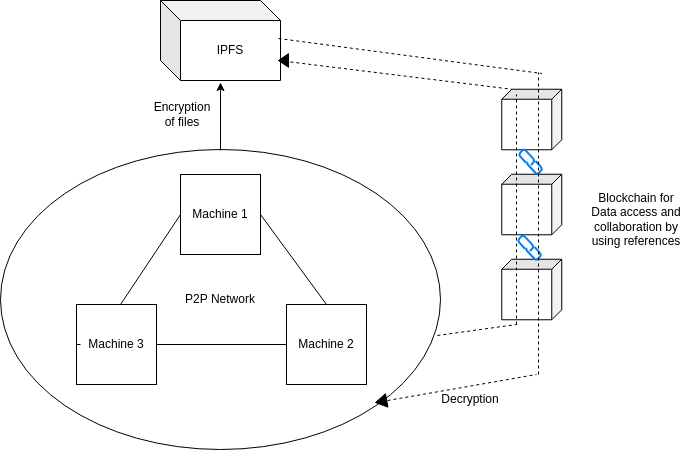
\includegraphics[width=14cm]{images/arch.png}
% \begin{center}
%     Proposed System Design
% \end{center}

\section{Dataset Description}

\noindent This research will be conducted using the HAM10000 ("Human Against Machine with 10000 training images") dataset \cite{tschandl2018ham10000}. This is a widely-used benchmark for dermatoscopic image classification, consisting of 10,015 multi-source dermatoscopic images of common pigmented skin lesions. The images are collected from different populations and modalities, representing a realistic clinical distribution. The dataset is classified into seven key diagnostic categories:

\begin{itemize}
    \item Actinic keratoses and intraepithelial carcinoma (akiec)

    \item Basal cell carcinoma (bcc)

    \item Benign keratosis-like lesions (bkl) (solar lentigines / seborrheic keratoses / lichen planus-like keratoses)

    \item Dermatofibroma (df)
 
    \item Melanoma (mel)

    \item Melanocytic nevi (nv)

    \item Vascular lesions (vasc) (angiomas, angiokeratomas, pyogenic granulomas and hemorrhage)
\end{itemize}

A significant challenge of this dataset is its severe class imbalance, with Melanocytic nevi (nv) comprising a majority of the samples. This imbalance necessitates the use of robust training strategies, such as weighted loss functions, class-aware sampling, and advanced data augmentation, to prevent the model from being biased towards the majority class. For our experiments, the dataset will be partitioned into training, validation, and testing sets with a standard 80-10-10 split, ensuring that the class distribution is stratified across all splits.
\section{Methodology}
The proposed methodology is a comprehensive three-phase pipeline, as detailed in previous chapters. Here we provide a structured overview:

\begin{enumerate}
    \item \textbf{Phase 1:} Self-Supervised Pre-training: A Vision Transformer (ViT-B/16) backbone will be pre-trained on the entire HAM10000 training set using the Momentum Contrast v3 (MoCo v3) framework. This will produce a set of weights that are highly adapted to the specific domain of dermatoscopic imagery.
    
    \item \textbf{Phase 2:} Teacher Model Training: The pre-trained backbone will be integrated into our novel Context-Aware Hierarchical Vision Transformer (CA-HVT). This teacher model will then be fine-tuned on the labeled training data in a fully supervised manner. The objective is to maximize diagnostic accuracy, creating an "expert" model that serves as the gold standard for knowledge distillation.
 
    \item \textbf{Phase 3:} Knowledge Distillation: The trained CA-HVT teacher model's knowledge will be transferred to a lightweight TinyViT student model. This will be accomplished using our proposed Attention-Guided Relational Knowledge Distillation (ARK-KD) framework. The student will be trained to mimic the teacher's logits, feature space geometry, and spatial attention patterns simultaneously.

    \item \textbf{Evaluation:} The final distilled student model will be rigorously evaluated on the held-out test set. We will report a comprehensive set of metrics, including overall accuracy, per-class F1-score, precision, recall, and balanced accuracy. We will also perform qualitative analysis using techniques like Grad-CAM to interpret the model's decision-making process.

\end{enumerate}
\section{Proposed Research Timeline}
\noindent The following table outlines the proposed timeline for the completion of this research thesis over a 12-month period.\\
    % \centering
    % 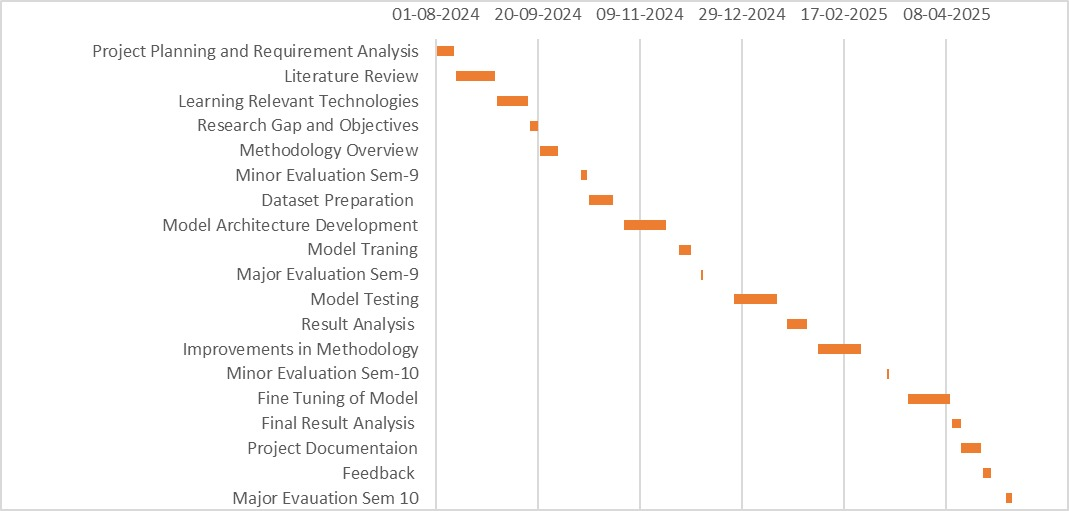
\includegraphics[width=16cm]{chapters/1/WhatsApp Image 2024-10-11 at 14.49.55.jpeg}



\begin{table}[h!]
\centering
\caption{Proposed Research Timeline}
\label{tab:gantt}
\renewcommand{\arraystretch}{1.4}
\begin{adjustbox}{max width=\textwidth}
\begin{tabular}{| p{6cm} | c | c | c | c | c | c |}
\hline
\textbf{Task} & \textbf{M 1-2} & \textbf{M 3-4} & \textbf{M 5-6} & \textbf{M 7-8} & \textbf{M 9-10} & \textbf{M 11-12} \\
\hline
1. Literature Review \& Finalizing Proposal & \cellcolor{gray!40} & & & & & \\
\hline
2. Data Preparation \& Pre-processing & \cellcolor{gray!40} & & & & & \\
\hline
3. Phase 1: SSL Pre-training & & \cellcolor{gray!40} & & & & \\
\hline
4. Phase 2: CA-HVT Teacher Implementation \& Training & & & \cellcolor{gray!40} & & & \\
\hline
5. Phase 3: ARK-KD Distillation Implementation \& Training & & & & \cellcolor{gray!40} & & \\
\hline
6. Model Evaluation and Results Analysis & & & & & \cellcolor{gray!40} & \\
\hline
7. Thesis Writing: Methodology \& Results Chapters & & & & \cellcolor{gray!40} & \cellcolor{gray!40} & \\
\hline
8. Thesis Writing: Introduction, Discussion \& Conclusion & & & & & & \cellcolor{gray!40} \\
\hline
9. Final Review and Thesis Submission & & & & & & \cellcolor{gray!40} \\
\hline
\end{tabular}
\end{adjustbox}
\end{table}

